\section{Intervention Context}

With the development of new technology described in the following section, interventions will be staged through Virginia Tech's new ``Introduction to Computational Thinking'' course, created to help fulfill the university's new General Education Requirements~\cite{vt-vision}. 
This course has already been run for two semesters, deeply incorporating much of my existing research work.
The course is taught and developed primarily by Dr. Dennis Kafura, although I have also been involved as associate instructor, managing course materials, server and technology administration, and assisting with in-class teaching.
However, now that the course is more solidly defined, my role is shifting into a more observational function in order to drive my dissertation work.
As a research endeavor, the course is heavily instrumented to provide data on its novel pedagogies and technologies.
Although there are confounding factors to working with such a heavily experimental course, it presents a unique testbed for materials and is an excellent source for mining research results.

\subsection{The Learners}

The students in the Computational Thinking course present a unique profile.
A few of them will have had prior programming experience, but most of them have had very minimal interactions with computers (indeed, they often describe themselves as ``not a computer person'').
These students may not believe that Computational Thinking will help them.
This is largely because they have more clearly defined domain identities, and may not see how Computational Thinking fits into them.
So, indeed, these students often have low motivation, especially in their sense of Success and Usefulness.

In the first offering of the course, 25 students enrolled in the course, and 20 students finished the coursework.
In the second offering, 40 students initially enrolled and 35 successfully passed the course.
Figure \ref{data-demographics} indicates the relevant demographic data collected through surveys.
Largely, the students represent the population at Virginia Tech, albeit with some disproportion towards certain majors than others.
It is worth pointing out the excellent gender diversity within the class.

\begin{figure*}
\begin{minipage}{\linewidth}
\centering
	\begin{tabular}{c|c|c}
	  \multicolumn{3}{c}{Gender}\\\hline
		& Fall 2014 & Spring 2015 \\\hline
		Female & 6 & 21 \\
		Male & 13 & 18 \\
	\end{tabular}
\centering
	\begin{tabular}{c|c|c}
	  \multicolumn{3}{c}{Prior Programming Experience}\\\hline
		& Fall 2014 & Spring 2015 \\\hline
		Yes & 10 & 7 \\
		No & 10 & 32 \\
	\end{tabular}
\centering
	\begin{tabular}{c|c|c}
		\multicolumn{3}{c}{Year}\\\hline
		& Fall 2014 & Spring 2015 \\\hline
		Freshman & 2 & 5 \\
		Sophomore & 7 & 11 \\
		Junior & 6 & 11 \\
		Senior & 5 & 10 \\
		Unknown & 0 & 2 \\
	\end{tabular}
\centering	
	\begin{tabular}{c|c|c}
	  \multicolumn{3}{c}{Colleges}\\\hline
		& Fall 2014 & Spring 2015 \\\hline
		Engineering & 2 & 2 \\
		Agriculture & 0 & 1 \\
		Sciences & 7 & 5 \\
		Liberal Arts & 9 & 23 \\
		Architecture & 1 & 7 \\
		Natural Resources & 0 & 0 \\
	\end{tabular}
\caption{Demographic Data of Computational Thinking Students}
\label{data-demographics}
\end{minipage}
\end{figure*}


\subsection{The Content}

Virginia Tech defines four learning objectives for ``Computational and Quantitative Thinking''~\cite{vt-vision}. Although the Computational Thinking only satisfies four of these objectives outright, they are all considered valuable end-goals:
\begin{enumerate}
	\item Explain the application of computational or quantitative thinking across multiple knowledge domains.
	\item Apply the foundational principles of computational or quantitative thinking to frame a question and devise a solution in a particular field of study.
	\item Identify the impacts of computing and information technology on humanity.
	\item Construct a model based on computational methods to analyze complex or large-scale phenomenon.
	\item Draw valid quantitative inferences about situations characterized by inherent uncertainty.
	\item Evaluate conclusions drawn from or decisions based on quantitative data.
\end{enumerate}

This content is mapped roughly into four instructional units on Computational Modelling, Algorithms, Data Intensive Inquiry, and Social Impacts. The lattermost unit is threaded throughout the course, while the first three are roughly sequential. Figure \ref{course-outline} gives a high-level overview of the content of this course.

\begin{figure*}
\begin{tabularx}{\textwidth}{ |l|X| }
\hline
Topic (Length) &	Description \\\hline
Computational Modeling \newline\newline
 (2 weeks) & Model-based investigation of how complex global behavior arises from the interaction of many “agents”, each operating according to local rules. Students use case-based reasoning and encounter basic computation constructs in a highly supportive simulation environment. \\\hline
Fundamentals of Algorithms \newline (4 weeks) & Study of the basic constructs of programming logic (sequence, decisions, and iteration) and program organization (procedures). A block-based programming language is used to avoid syntactic details. Students can see how these constructs are expressed in Python. \\\hline
Data-intensive Inquiry \newline (7 weeks) & Project-based exploration of complex phenomena by algorithmically manipulating large-scale data from real-world sources. Students construct algorithms in Python using a supportive framework for accessing the data. \\\hline
Social Impacts \newline (2 weeks) & Explore and discuss contemporary societal issues involving computing and information technology. \\\hline
\end{tabularx}
\caption{High-Level Course Overview}
\label{course-outline}
\end{figure*}

It is clear that this material aligns smoothly with the content described in this preliminary proposal, in particular a focus on algorithms and abstraction.

\subsection{The Course}

The course uses a considerable amount of modern pedagogical techniques, many of which represent ongoing research questions.
Perhaps the most influential technique is the organization of students into cohorts.
Near the beginning of the semester, students are put into groups of 5-6, balancing based on year and gender where possible, and avoiding putting similar majors into the same group.
These cohorts primarily function as a support structure that students can rely on to get help and encouragement.
Although cohorts work together on many smaller in-class assignments, every student is ultimately responsible for their own work -- the final project, for instance, is individual to each student.

Class time is split between presentation (typically stand-up lecture) and participation (typically computer-based work or cohort discussion) using an Active Learning style whereever possible.
Earlier questions in the course often have students completing questions on paper or doing more kinetic exercises.
Later questions rely on the automated Kennel questions, until the students reach the open-ended project work.

Work in the class is considered to be under a mastery style -- deadlines are enforced only in so far as they motivate students to complete assignments, not in order to punish.
Students are free to work on the material as long as they need.
A recurring message within the course is that ``failing is okay, as long as you keep trying''.

\section{Research Questions}

In this section, I outline the research problems that I will explore.

\subsection{The Use of Datasets}

\textbf{What are the issues using datasets, and how do we manage them?}

In this section, I outline a number of the biggest issues in using datasets as an introductory context.
Existing research in this area is largely concerned with providing examples of how to use datasets, rather than solving these more generalized problems.
I will develop meaningful classifications, theories, guides, and materials to help instructors and course developers manage these issues.

\subsubsection{Preparation of Datasets}

One of the most general questions when it comes to these datasets is how to organize and prepare the dataset. Where should the data come from? Data can be collected by organizations, by the instructor, by the students (e.g., using data in their own lives), or any of a number of different sources. That data can be based on a simulation or predicted model (e.g., fantasy football), or observations of a real phenomenon (e.g., weather reports)? I will analyze these different sources, the affordances and costs associated with them, and develop conclusions on the best way to leverage them. This will include guides on how to find and develop datasets.

\subsubsection{Normalization of Difficulty}

An incredibly useful problem to solve is how to meaningfully normalize difficulty between datasets and identify the difficulty of a given dataset. If this could be accomplished, instructors could confidently empower students to pursue distinct projects while ensuring that they are having a mostly uniform experiences. Difficulty creeps through in a number of ways, as described in the following list. \begin{description}
	  \item[Domain Knowledge Required:] Understanding a dataset requires the student to understand the greater context, entities, relationships, and reality that the dataset abstracts. In some cases, students (especially in Computational Thinking) bring useful prior knowledge that help them to rapidly comprehend a dataset. When this knowledge is not present, an extra level of difficulty is added. For example, in the Computational Thinking class, students easily grasped the Weather dataset (featuring an abstraction of temperature as a number), but struggled with the Stock Value dataset (featuring an abstraction of stock values as numbers) -- even though both datasets had the exact same data structure.
		
		However, there are other ways that domain knowledge can be a problem -- students' prior knowledge can be limited, incorrect, or difficult to leverage, for example. I will describe best practices for helping students get to know datasets and identifying whether a dataset is suitable for a given student or sets of students.
		\item[Computing Knowledge Required:] Anyone making a dataset must become familiar with how to structure the data. Anyone using a dataset must become familiar with how to process it. Any programming interfaces made available (e.g., special libraries and frameworks) incur their own costs. Although some languages are made specifically to handle data processing using high-level declarative techniques (e.g., SQL), other languages require different levels of specificity on how to manipulate the data. In a practical setting, there are major advantages to choosing the ``simplest'' option (one might argue, for example, that a declarative language makes filtering easier than a functional language does, and a functional language makes filtering easier than a imperative language does). However, when the goal is to teach concepts, there may be other advantages related to the learning objectives to using these datasets. I will analyze and describe the pedagogical affordances that different data structures and programming styles create.
		
		Included in this analysis is research on the effectiveness of the Block-based Programming Environment for guiding students to work with datasets.
		As previously mentioned, the Block-based environment used in the Computational Thinking course has first-order support for integrating datasets. However, there are open questions as to how effective the environment is in teaching students.
		I will expand and evaluate the Block-based Environment's capabilities for supporting students understanding of working with datasets and the introductory computing content.
		
		\item[Dataset Knowledge Required:] In general, learning to work with a new dataset requires time and attention to become familiar with its particular structure and design. Why was it organized the way it was (e.g., as a list of dictionaries as opposed to a dictionary of lists).
	\end{description}
		Understanding the structure, meaning, and values of data can be a difficult problem for introductory students.
		Using Data Science as the introductory context puts an increased emphasis on data structures and algorithms, making this content more critical for the learner.
		Currently, there are not many tools available to scaffold students in getting to know datasets.
		An example of a possible approach is Spyder's Variable Explorer, seen in figure \ref{fig-spyder-explorer}, which allows users to drill-down through a data structure (assuming it uses native Python \texttt{list}s and \texttt{dict}s) by opening nested windows. 
		Although this tool is powerful, it is limited pedagogically by offering very little supplementing knowledge.
		However, it does provide a useful example of a way to visually explore a dataset.

		A number of graphical representations are used throughout the Computational Thinking course in order to visualize topics such as Abstraction and program flow.
		For instance, students build Data Map Diagrams as seen in Figure \ref{data-maps-weather}, intended to help them navigate complex data structures.
		A system will be created to generate simplified graphical visualizations of the students code and the data model in order to connect to these other course topics.
		The system will be available for data used in the course regularly, and should be extremely beginner-friendly.
		
		On the other hand, guidance will be created for dataset developers and instructors to adjust the structure and content of a dataset to normalize its difficulty.
		For example, a highly-nested dataset can be semi-automatically adjusted to drop levels of nesting in favor of a flatter structure.
		Alternatively, a list datapoints could be grouped by one of their features to make it easier to conduct grouped analysis (e.g., grouping weather reports by city or year so it is easier to calculate averages).
		There are a wide range of techniques that could be suggested based on a situation -- automatic analysis of the dataset could help provide suggestions on where the complexity can be increased, decreased, or aligned with specific learning objectives. 
		
\subsubsection{Reliability of the Dataset} There are a number of issues that the student and instructor should become aware of about the nature of the data, as a secondary concern. Was the data collected correctly? Were mistakes made in processing it? Are the abstractions false? Although some instructors may not find it a primary learning objective, students need to be aware of the possibilty of mistakes in the process of preparing a dataset, and instructors need to be aware of the ethical ramifications of presenting a dataset as reliable or authentic.
	
Careful consideration must be made when choosing problems and designing contexts so that the data leads to optimally authentic learning experiences.
In practice, datasets can vary greatly in authenticity -- some data is collected incorrectly or has other errors, some data was predicted from a model rather than observed from real phenomenon.
A curious component of authenticity, however, is that it is a function of the observer.
A persuasive instructor might convince a class of students that an entirely artificial dataset was representative of real-world data, especially if it confirmed students' existing biases.
There are ethical issues with artificial datasets and the stories that they tell.
However, there are serious pedagogical benefits to generating datasets that fit instructor's goals -- data that leads to interesting visualizations, or clean results.
An important facet of my research will be exploring the ethical and pedagogical ramifications of the authenticity of datasets.

One of the big dangers when attempting to create meaningful context for learners is the problem of \textit{Preauthentication}: attempting to design for authenticity without sufficient knowledge of the audience. This is a problem shared by any approach to introductory material. Petraglia gives a compelling example \cite{preauthentication}:
	
\begin{quotation}
    The task of balancing a checkbook, for instance, may be an authentic task from the perspective of a 21-year-old, but we would question its authenticity from the perspective of a 5-year-old. But more to the point, even among 21-year-olds, for whom we believe the task should be authentic, there are some who will find any given lesson in personal finance irrelevant, inaccurate, or otherwise inappropriate. 
\end{quotation}
Preauthentication stems from over-generalizations and run-away assumptions.
If you attempt to reduce an entire classroom to a list of likes and dislikes, you run the risk of ignoring each individual learner's rich history and background that they will be building from. 
It is difficult to plan for and work against this ever-present danger when designing reusable assignments. 
Petraglia \cite{preauthentication} recommends that rather than attempting to design around students prior understanding, it is better to simply convince the learner of the authenticity of the problem.
But this is limiting, since it ignores the prior experiences and understanding that a student brings to their learning.
Instead, it would be better to find a middle ground where students are given flexibility while maintaining a relatively uniform experience for students.
In an ideal learning environment, students will have freedom to explore datasets of their own choosing, possibly from a list.
Of course, this must be balanced with the students inexperience with finding datasets, requiring the process be given time and attention.
	
\subsubsection{Availability of the Dataset}

Some organizations make their data available only through certain channels -- students have to sign a legal agreement, or register for an API key. Organizations such as FERPA and HIPPA exist in order to ensure the privacy and dignity of captive populations (e.g., school children, patients). These organizations define rules for how data on such populations can be published and made available. Often, interesting data exists behind walled gardens. Although novel techniques such as Differential Privacy (where data is probabilistically modified to protect anonymity~\cite{dwork2011differential}) can be used to mitigate these problems, it is simply a fact that some data is utterly unaccessible. I will explore the options available to mitigate the dataset, and their affect on the authenticity of the data.
	
	Of course, the format of the dataset itself may lead to unavailability. Many developers have limited experience, time, and interest with the best way to package data for others' consumption, especially when it comes to beginners. It can be easy to release a dataset as a PDF or in some obscure binary format. Overtime, data can also disappear behind dead/moved URLs. A major challenge for organizing data can be finding it and interpreting it. I will analyze the common pitfalls committed in releasing data to develop preventive and corrective measures.

\subsubsection{Other Motivational Value of the Dataset}

A given dataset has some motivational value that is a function of the student, the context, and the dataset itself. Although Goldweber et al ~\cite{SocialGoodinComputingEducation} attempted to define these elements in a general sense, there is no coherent model to holistically describe how motivation is imparted in datasets. I will analyze the factors and elements of a motivation and derive a detailed framework for evaluating the motivational value of a dataset. Examples of the kinds of issues present in this question are:\begin{description}
		\item[Interestingness of the Dataset:] Does the dataset have generalized appeal, or is it more niche?
		\item[Freshness of the Dataset:] Has this dataset been explored before? Have people already used it to answer questions?
		\item[Usefulness of the Dataset:] Does the dataset hold the answers to any questions? Is getting results from it like pulling water from a stone? How much work is required to answer these questions -- is it a problet or a project?
		\item[Social Nature of the Dataset:] Does the dataset relate to a real-world problem? Or is it more esoteric or socially (lowercase S) natured?
	\end{description}
	
\subsubsection{Comparison of the Context} As outlined in section 3, there are a number of different contexts available to instructors. What makes data science a particularly effective one, compared to the alternatives? I will conduct surveys of students in order to find out how they compare from their perspective. The goal of this research question is to find out the trade-offs and value of this context, and whether it can be a true all-in-one.

\begin{figure}[!ht]
\label{fig-spyder-explorer}
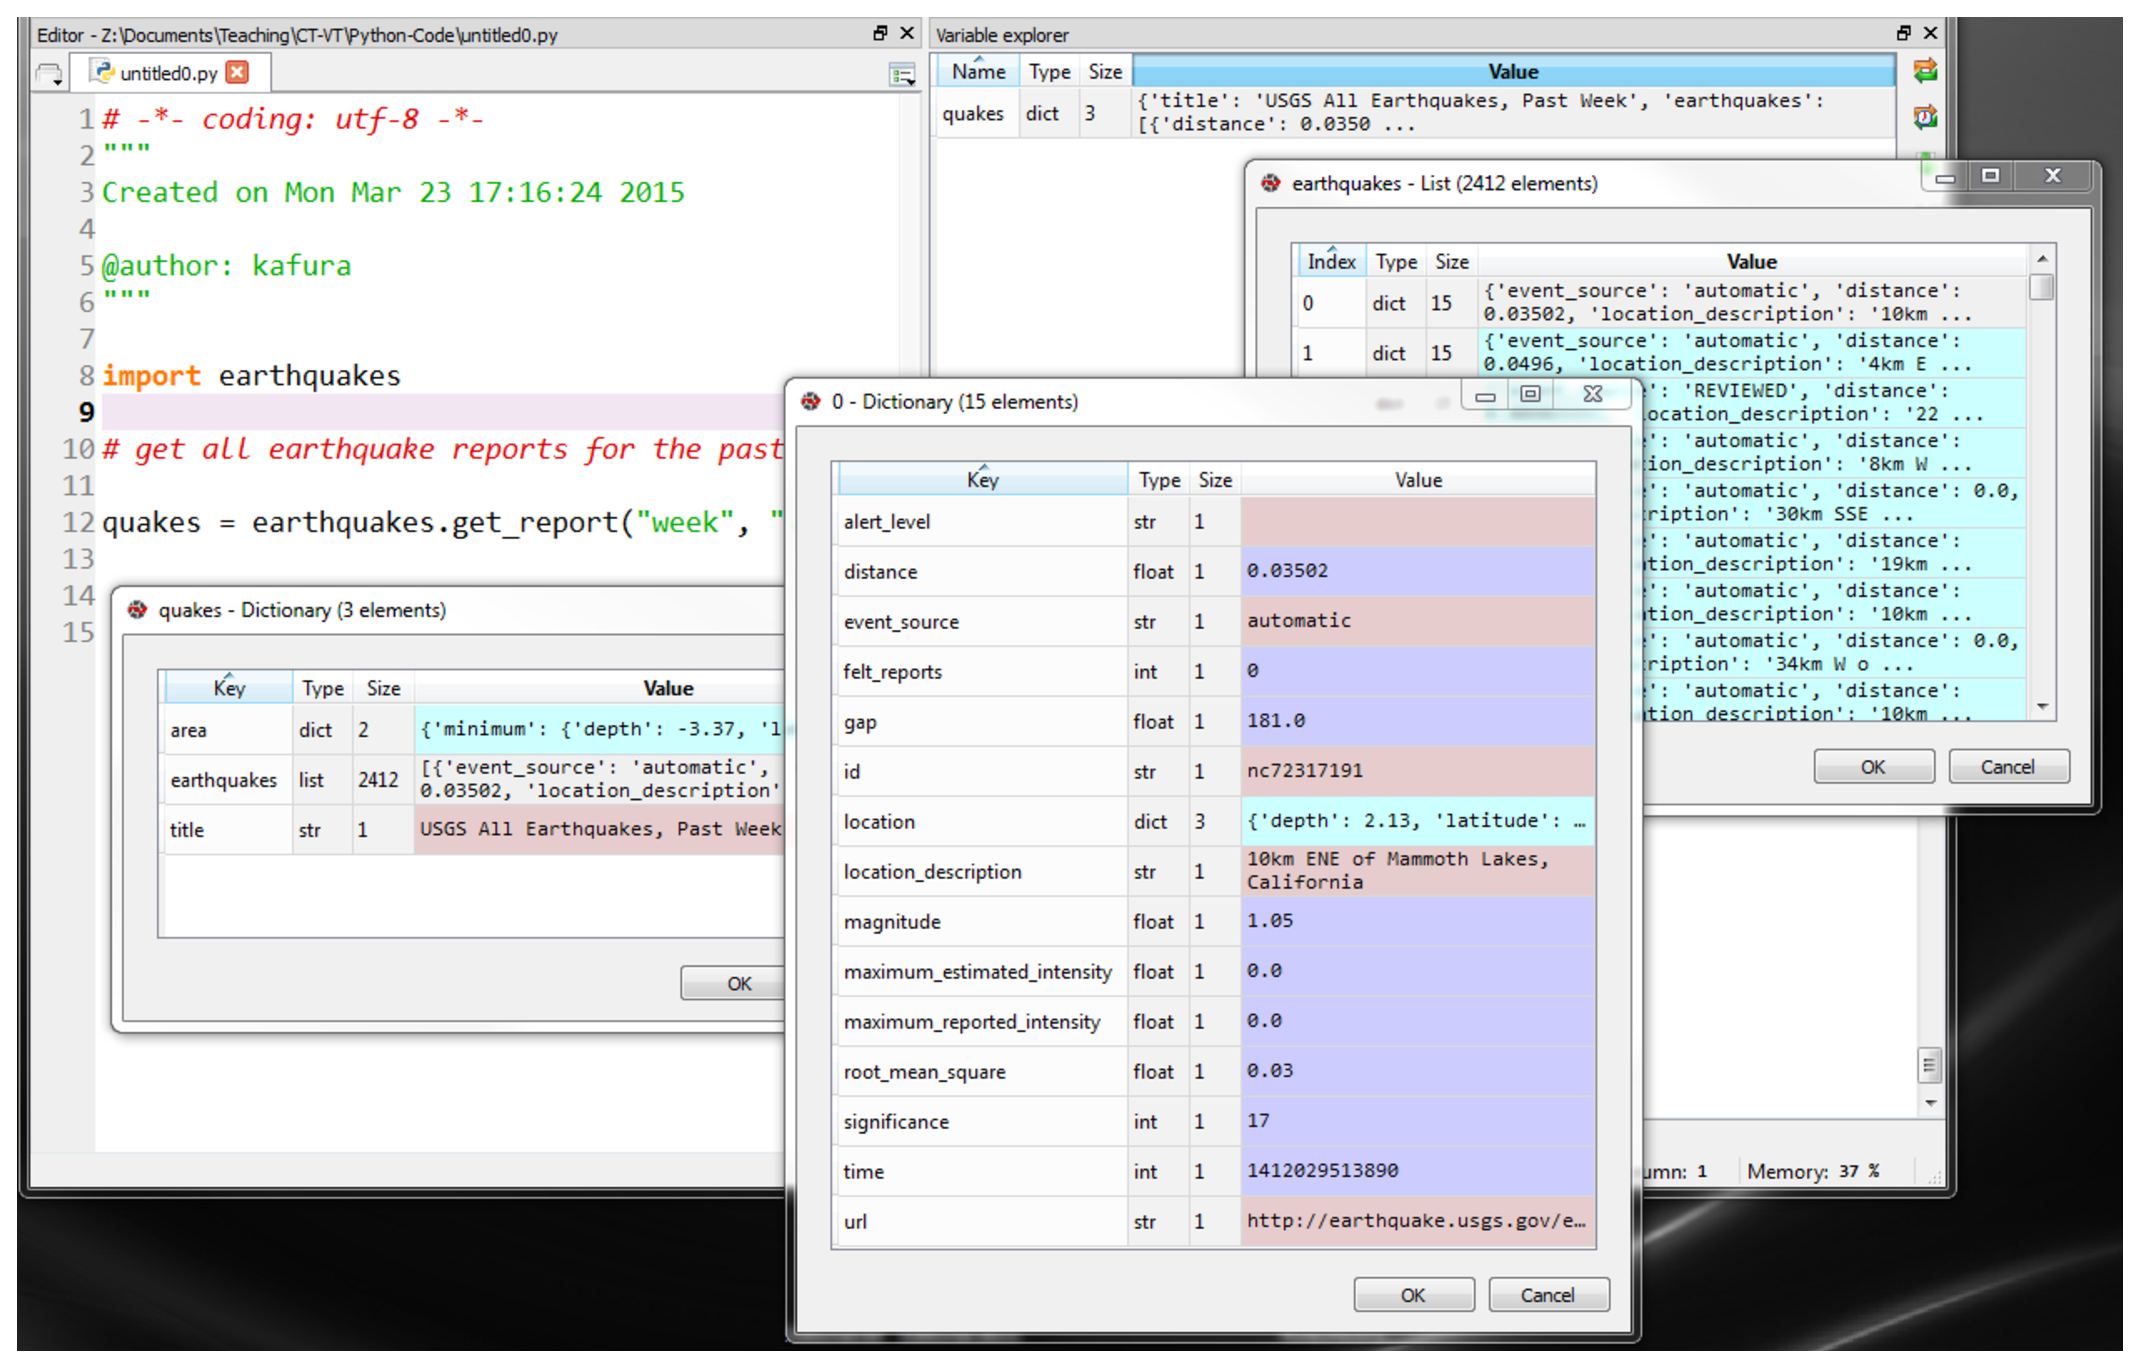
\psfig{file=images/spyder-explorer.eps, width=\linewidth}
\caption{The Spyder Programming Environment for Python has a Powerful Variable Explorer Tool}
\end{figure}

\subsection{Academic Motivation and Learning?}
There is strong evidence that motivation predicts performance in the course, and my research will contribute to this growing base.
Motivation in the course will be primarily assessed through self-reported surveys based heavily on the MUSIC Model of Academic Motivation Inventory (MMAMI).
Students will be non-anonymously surveyed using the complete instrument at key points in the semester, and regularly surveyed using a miniaturized version throughout the semester.
These miniaturized versions will be used as follow-ups to specific course exercises in order to determine more finely-grained answers about where students found motivation.
Additionally, targeted qualitative data will be gathered in order to refine this quantitative data.

This motivational data will be combined with evidence of engagement with the course across several different dimensions. Therefore, the complete list of motivational sources is:
\begin{description}
	\item[Attendance:] Did the students regularly attend class?
	\item[Retention:] Did the students complete the course with a passing grade?
	\item[Coursework:] Did the students regularly complete coursework and homework on time?
	\item[Struggle:] Did the students continue with materials even after setbacks?
	\item[Continuation:] Do students intend to follow-up the course with further courses and learning experiences in Computational Thinking?
	\item[Observations:] Did the course staff report students as being motivated, according to their own observations? In Spring 2014, for example, teaching assistants were asked to rank their students on a scale of 1--4 to indicate how engaged they were.
	\item[Self-report:] Did the students report themselves as being motivated, according to MMAMI and other surveys?
	\item[Success:] Did the students succeed at the final project and overall course?
\end{description}
This evidence, along with the MUSIC model's data, can be used to explore academic motivation within Computer Science more holistically.

\subsection{Extension of Materials}

\textbf{How can we disseminate the research materials and results I am developing?}

The CORGIS project depends on having an extensive and varied collection of datasets. 
Students should be able to find a dataset that appeals to their personal interests but provides a sound learning experience.
Making this experience relatively uniform is challenging, but makes providing support much easier -- a necessary element in a scaled classroom.

The same data source can be expressed in many ways, representing different levels of abstraction and different affordances.
Consider the data map in figure \ref{data-maps-weather}, representing potential structures for weather data collected about cities around the world.
Although maps A and B contain the exact same data, they are structured very differently -- a list of cities vs. a dictionary of cities.
For an experienced programmer, these differences are minor details that have implications for runtime performance: looking up a city's temperature is slower and more complicated in structure A (requring iteration and decision) than it is in B (requiring only dictionary access).
Although the differences in code are minor to an expert, they require fundamentally different areas of knowledge for a beginner.
Map C represents an entirely different level of abstraction, where weather is only represented as a numeric, without information about cities.
The number of questions that can be answered using this data is greatly reduced -- statistics about cities in general, rather than comparisons against specific cities.
And of course, the nature and schema of the data itself affects the types of questions that can be asked -- it makes sense to find the average of a list of temperatures, but not the sum.
A key part of my research will be explicitly identifying trade-offs and affordances of different structures and abstractions of data.

\begin{figure}
\begin{center}
\tikzset{
    bnode/.style = {   
        align=center, draw,
        rectangle split, rectangle split horizontal,
				rectangle split draw splits=false
    }
}
\begin{minipage}{.4\textwidth}
\begin{tikzpicture}
    \node[align=center, draw] (root)
		  {List of}
		;
		\node[bnode, below=of root,rectangle split parts=3]
       (middle)
       {	\nodepart{one}
					Dictionary of:
					\nodepart{two}
          ``city'' ,
					\nodepart{three}
					``temperature''
					};
		
    \draw (root) -- (middle);
    \draw (middle.two south) -- +(0, -1) node[draw, anchor=north](q) {string};
    \draw (middle.three south) -- +(0, -1) node[draw, anchor=north](q) {integer};
		%  +(0,-1) 
\end{tikzpicture}
\begin{center}
(A) List of Weathers
\end{center}
\end{minipage}
\begin{minipage}{.4\textwidth}
\tikzset{
    bnode/.style = {   
        align=center, draw,
        rectangle split, rectangle split horizontal,
				rectangle split draw splits=false, rectangle split parts=4
    }
}
\begin{tikzpicture}
		\node[bnode]
       (root)
       {	\nodepart{one}
					Dictionary of:
					\nodepart{two}
          ``blacksburg'' ,
					\nodepart{three}
					``newark'',
					\nodepart{four}
					``venice''
					};
		
    \draw (root.two south) -- +(0, -1) node[draw, anchor=north](q) {integer};
    \draw (root.three south) -- +(0, -1) node[draw, anchor=north](q) {integer};
		\draw (root.four south) -- +(0, -1) node[draw, anchor=north](q) {integer};
		%  +(0,-1) 
\end{tikzpicture}
\begin{center}
(B) Dictionary of Weathers
\end{center}
\end{minipage}


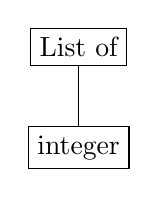
\begin{tikzpicture}
		\node[align=center, draw] (root)
		  {List of}
		;
		
    \draw (root) -- +(0, -1) node[draw, anchor=north](q) {integer};
		%  +(0,-1) 
\end{tikzpicture}
\begin{center}
(C) List of Temperatures
\end{center}

\end{center}
\caption{Weather Data Maps}
\label{data-maps-weather}
\end{figure}

Finding data sources can be a challenging task.
A component of my research plan is to publish best practices and techniques for finding, organizing, and exposing datasets.
The CORGIS collection already contains three dozen libraries, covering areas as diverse as international studies, nutrition, and social media platforms.
Some datasets were chosen because they were low-hanging fruit -- extensively documented, freely available, and well-supported. 
However, other datasets were driven by students' needs; in the two semesters that the course has been offered, two dozen new datasets have been created on demand.
The rapid turn-around time required has given new insight into the process of data mangling, although I am still exploring methods.
A massive part of my proposed work is to solidify and publish these techniques into a full paper.

In addition to guides on the development of datasets, I will create guidance on how to meaningfully integrate these materials at multiple levels of a course.
Drawing on principles of Instructional Design, I will create materials that are quickly adaptable to courses at the problem-level and the project-level.
Instructors will be provided with guides on how to integrate these datasets into their courses most meaningfully.